\documentclass{beamer}

 \usepackage[german]{babel}
 \usepackage[utf8]{inputenc}
 \usepackage{graphicx}
\usetheme{Boadilla}

\setbeamercovered{transparent}
\beamertemplatenavigationsymbolsempty
\setbeamertemplate{footline}[frame number]

\title[Rapi]{Raspberry Pi ROS}
\author[D. Herdt, A. Causevic]{Dennis Herdt, Almin Causevic}
\institute[I_HS Wgt-Rav]{Informatik HS Weingarten-Ravensburg}
\date{\today}
%\logo{\pgfimage[width=2cm,height=2cm]{hulogo}}
%\titlegraphic{\includegraphics[width=2cm,height=2cm]{hulogo}}
\subject{Raspberry Pi ROS}

\begin{document}

\begin{frame}[fragile]
%\begin{figure}[h]


\includegraphics[width=2cm]{pics/hs-logo.jpg}
%\end{figure}


\vspace{1cm}

\begin{center}

{\bf \huge ROS auf dem Raspberry Pi}
\vspace{2cm}

\today

\end{center}
\end{frame}

\begin{frame}
\centerline{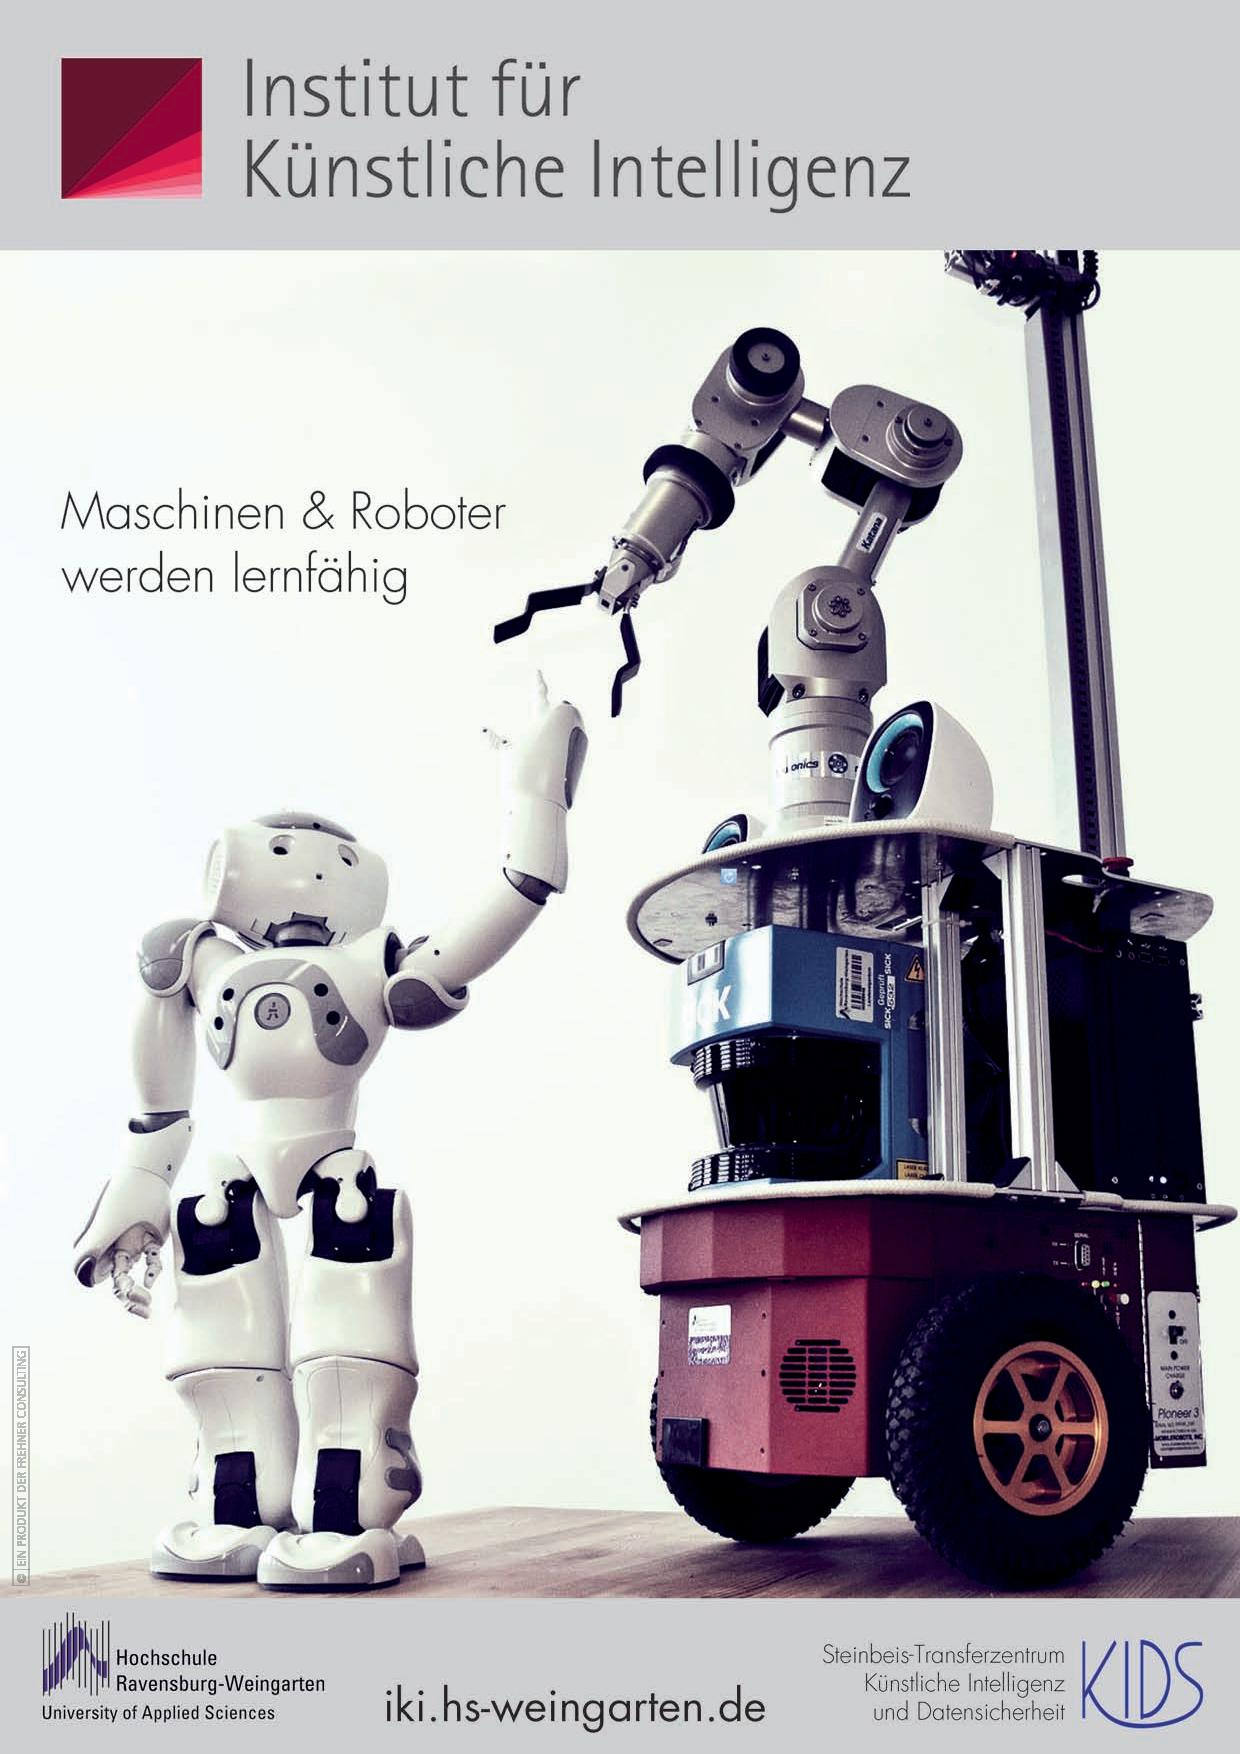
\includegraphics[width=6cm]{pics/iki.jpg}}
\end{frame}

\begin{frame}
\centerline{
\includegraphics[width=6cm]{pics/ros5.png}}
\end{frame}

\begin{frame}
\centerline{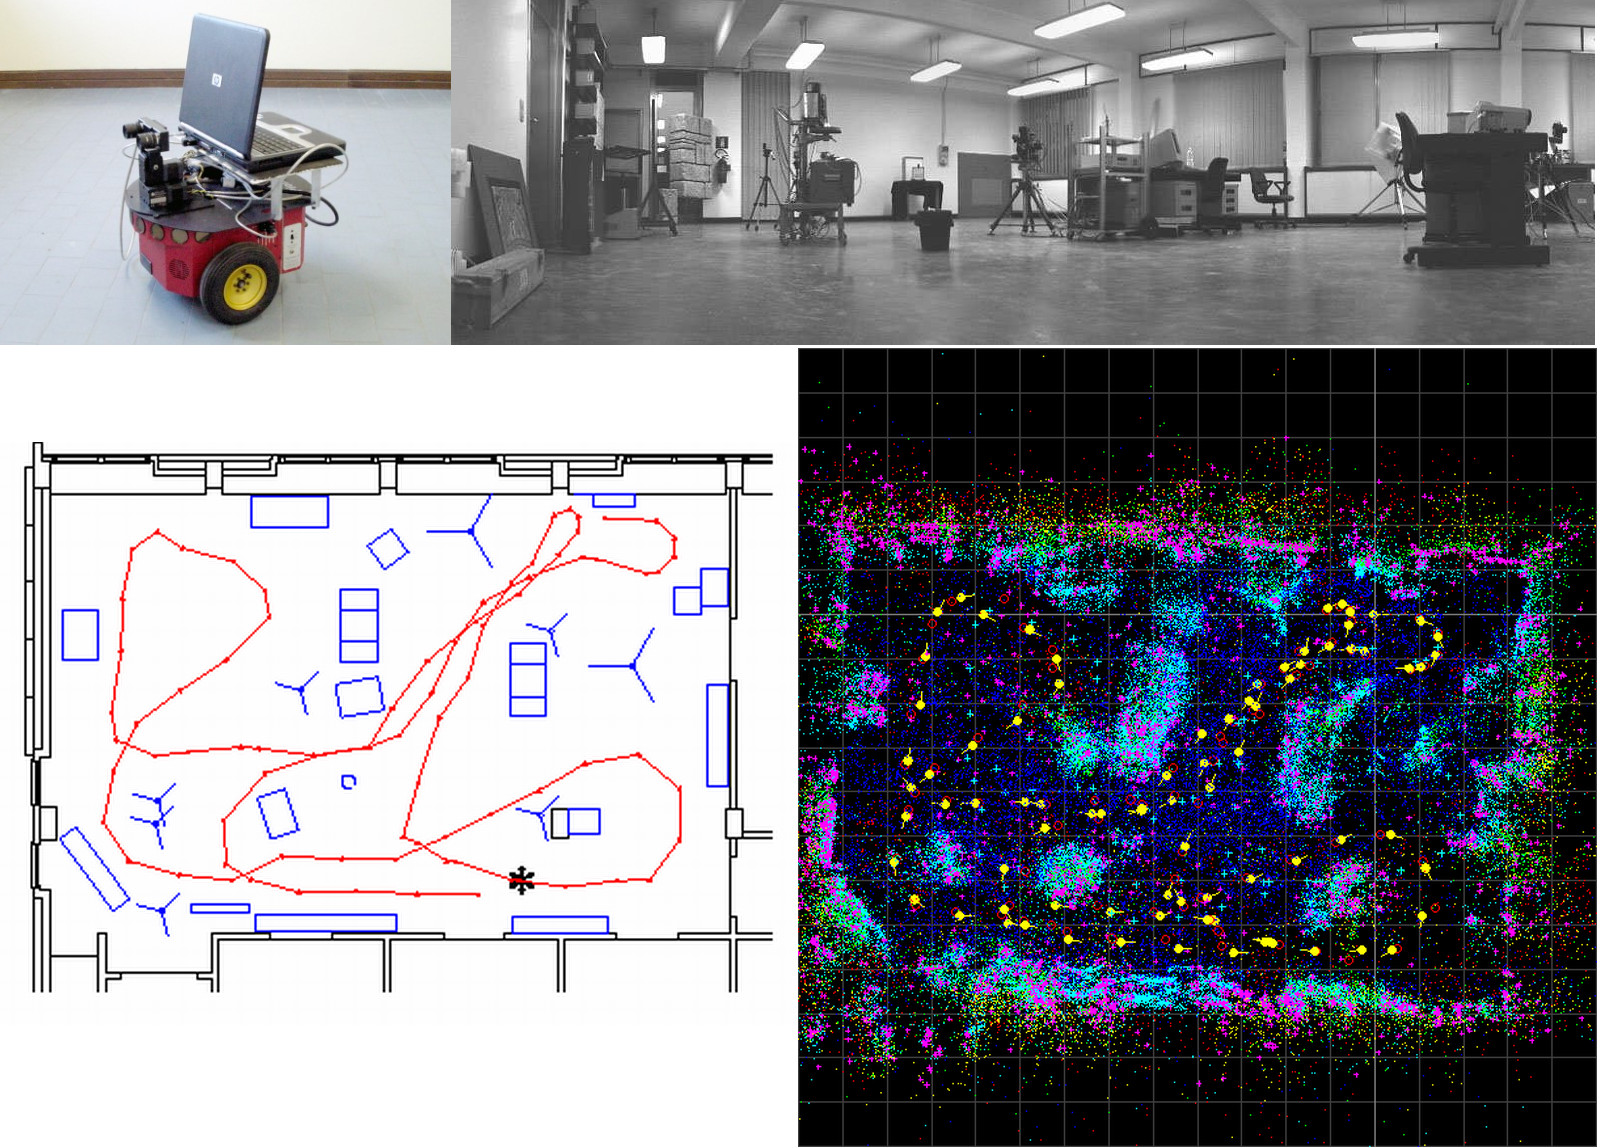
\includegraphics[width=6cm]{pics/slam.png}}
\end{frame}

\begin{frame}
\centerline{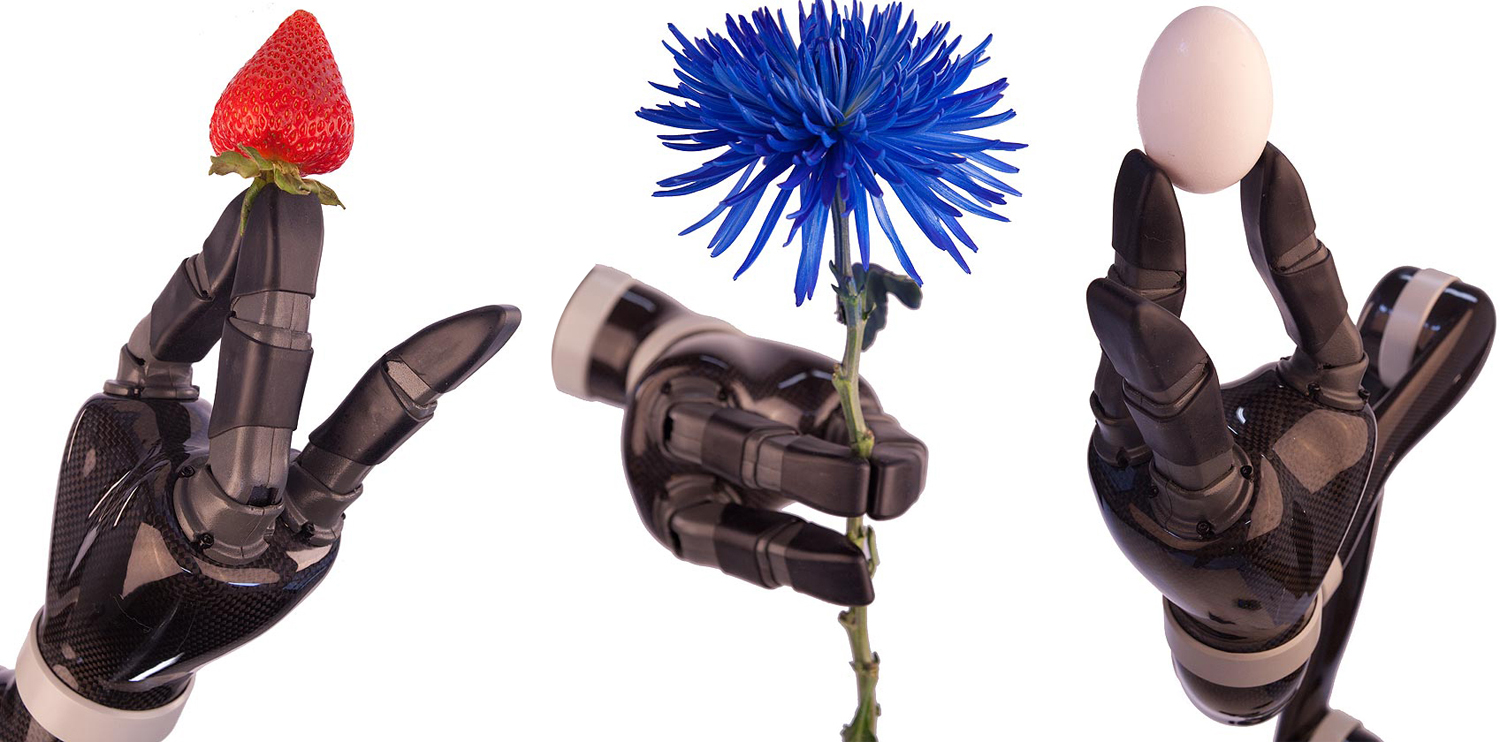
\includegraphics[width=6cm]{pics/jaco_arm.jpg}}
\end{frame}

\begin{frame}
\parbox{5cm}{
\includegraphics[width=3cm]{pics/carmen.png}}
\parbox{5cm}{
\includegraphics[width=3cm]{pics/yarp.png}}
\parbox{5cm}{
\includegraphics[width=3cm]{pics/microsoft.jpg}}
\hspace{5cm}
\parbox{5cm}{
\includegraphics[width=3cm]{pics/orocos.jpg}}
\parbox{5cm}{
\includegraphics[width=3cm]{pics/orca.png}}
\end{frame}

\begin{frame}
\centerline{
\includegraphics[width=12cm]{pics/ros_equation.png}}
\end{frame}

\begin{frame}
\centerline{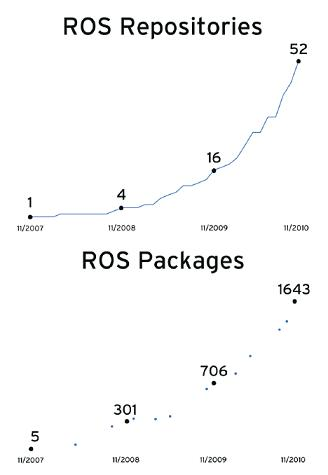
\includegraphics[width=6cm]{pics/ros_repos.jpg}}
\end{frame}

\end{document}
